\documentclass{standalone}

\usepackage{circuitikz}

\begin{document}

% INT_AY22_L28-Fig17_Swirly_E_field.png

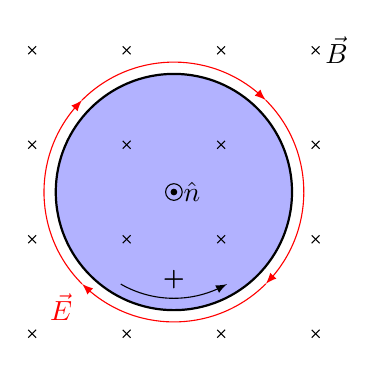
\begin{tikzpicture}[> = latex]

	% Definition
	
	\def\R{1.65} 		% Size of electric field line

	% Circle with thick boundary
	
	\filldraw [thick, draw = black, fill = blue!30] (0, 0) circle (1.5 cm);
	
	% Non-conservative electric field
	
	\draw [red, ->] (135 : \R) arc (135 : 45 : \R);
	\draw [red, ->] (45 : \R) arc (45 : -45 : \R);
	\draw [red, ->] (315 : \R) arc (315 : 225 : \R) node [below left] {${\vec E}$};
	\draw [red, ->] (225 : \R) arc (225 : 135 : \R);
	
	% Normal vector
	
	\filldraw (0, 0) circle (1 pt);
	\draw (0, 0) circle (3 pt) node [right] {${\hat n}$};
	
	% Positive direction around loop
	
	\draw (240 : 1.35) arc (240 : 270 : 1.35) node [above] {$+$}; 
	\draw [->] (270 : 1.35) node [above] {$+$} arc (270 : 300 : 1.35);
	
	% Magnetic field
	
	\foreach \x in {-1.8, -0.6, 0.6, 1.8}
	\foreach \y in {-1.8, -0.6, 0.6, 1.8}
	{
		\draw (\x + 0.05, \y + 0.05) -- (\x - 0.05, \y - 0.05);
		\draw (\x + 0.05, \y - 0.05) -- (\x - 0.05, \y + 0.05);
	}
	
	\node [right] at (1.8, 1.8) {${\vec B}$};

\end{tikzpicture}

\end{document}